This section describes the subsystems within the Output Layer, responsible for providing user feedback through visual and audio channels.

\begin{figure}[h!]
	\centering
 	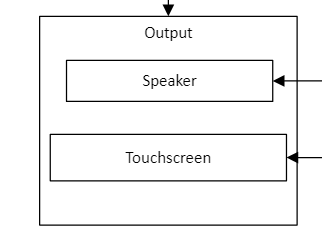
\includegraphics[width=0.60\textwidth]{images/OutputSubsystem}
 \caption{Example subsystem description diagram}
\end{figure}

\subsection{Speaker}
The speaker subsystem connected to the Sound Multiplexer

\subsubsection{Assumptions}
\begin{itemize}
\begin{item}
The Speaker subsystem receives analog signals from the Sound Multiplexer
\end{item}
\begin{item}
The Speaker subsystem is responsible for converting the analog signals into audible sound.
\end{item}
\end{itemize}

\subsubsection{Responsibilities}
\begin{itemize}
\begin{item}
Receive analog signals representing the final sound output from the Sound Multiplexer 
\end{item}
\begin{item}
onvert the analog signals into audible sound
\end{item}
\end{itemize}

\subsubsection{Subsystem Interfaces}

\begin {table}[H]
\caption {Subsystem interfaces} 
\begin{center}
    \begin{tabular}{ | p{1cm} | p{6cm} | p{3cm} | p{3cm} |}
    \hline
    ID & Description & Inputs & Outputs \\ \hline
    \#1 & Representing the final sound output from the Sound Multiplexer&Analog signals representing the final sound output & Audible sound  \\ \hline
    \end{tabular}
\end{center}
\end{table}

\subsection{Touchscreen}
The Touchscreen subsystem connected to the Control Unit
\subsubsection{ASSUMPTIONS}
\begin{itemize}
\begin{item}
The Touchscreen subsystem receives digital signals from the Control Unit
\end{item}
\begin{item}
The Touchscreen subsystem is responsible for displaying visual information to the user.
\end{item}
\end{itemize}
\subsubsection{RESPONSIBILITIES}
\begin{itemize}
\begin{item}
Receive digital signals from the Control Unit representing the visual information to be displayed
\end{item}
\begin{item}
Display the received information on the touchscreen
\end{item}
\end{itemize}

\subsubsection{SUBSYSTEM INTERFACES}

\begin {table}[H]
\caption {Subsystem interfaces} 
\begin{center}
    \begin{tabular}{ | p{1cm} | p{6cm} | p{3cm} | p{3cm} |}
    \hline
    ID & Description & Inputs & Outputs \\ \hline
    \#1 & The Touchscreen subsystem receives digital signals from the Control Unit & \pbox{3cm}{Digital signals representing visual information} & \pbox{3cm}{Visual information displayed on the touchscreen}  \\ \hline
    \end{tabular}
\end{center}
\end{table}